% Discusión de la réplica (se incluye en el informe). Los números salen de resultados.tex.
\subsection{Comparación con el artículo y causas de las diferencias}

\textbf{Valor absoluto.} El ConvMixer-128/8 llegó a \pct{\accCMnueve} en test, frente a \pct{95,0} que informa
el artículo para la misma configuración de núcleo y parche ($k=9$, $p=2$) con ancho 256. La diferencia de unos
12 puntos tiene causas concretas:
\begin{enumerate}
  \item \emph{Entrenamiento 20 veces más corto} (\epocasCNN{} épocas frente a 200). La Figura~\ref{fig:curvas}
  muestra que la validación se estabiliza en las últimas épocas sólo porque la tasa de aprendizaje llega a cero,
  no porque el modelo haya terminado de aprender.
  \item \emph{Modelo 3 veces más chico} (223\,k frente a 709\,k parámetros). En la Tabla~4 del artículo, pasar de
  $h=256$ a $h=128$ cuesta entre 1 y 2 puntos aun con 200 épocas.
  \item \emph{Sin RandAugment, mixup ni CutMix.} Según la Tabla~3 del artículo, quitar sólo RandAugment cuesta
  3 puntos.
  \item \emph{Protocolo más estricto}: el test se miró una sola vez y los hiperparámetros no se ajustaron sobre él.
\end{enumerate}

Para comprobar que la brecha se debe al cómputo y no a un error de implementación, entrené además el modelo en una
GPU gratuita de Google Colab (Tesla T4) con la receta del repositorio oficial de los autores para CIFAR-10
(\url{https://github.com/locuslab/convmixer-cifar10}): ConvMixer-256/8 con $k=5$ y $p=2$, RandAugment, ColorJitter,
\emph{random erasing} y 100 épocas, a unos \segColab{} segundos por época. Esa corrida llegó a \pct{\accColab} en test
\colabNota{} (Figura~\ref{fig:colab}). El artículo informa \pct{95,21} para esa configuración con 200 épocas. Es decir: con la receta
completa la implementación queda a menos de un punto del valor publicado, y la diferencia de la réplica en CPU se
explica por la escala del experimento.

\begin{figure}[h]
\caption{Réplica en GPU con la receta oficial de los autores (Google Colab, Tesla T4)}
\label{fig:colab}
\centering
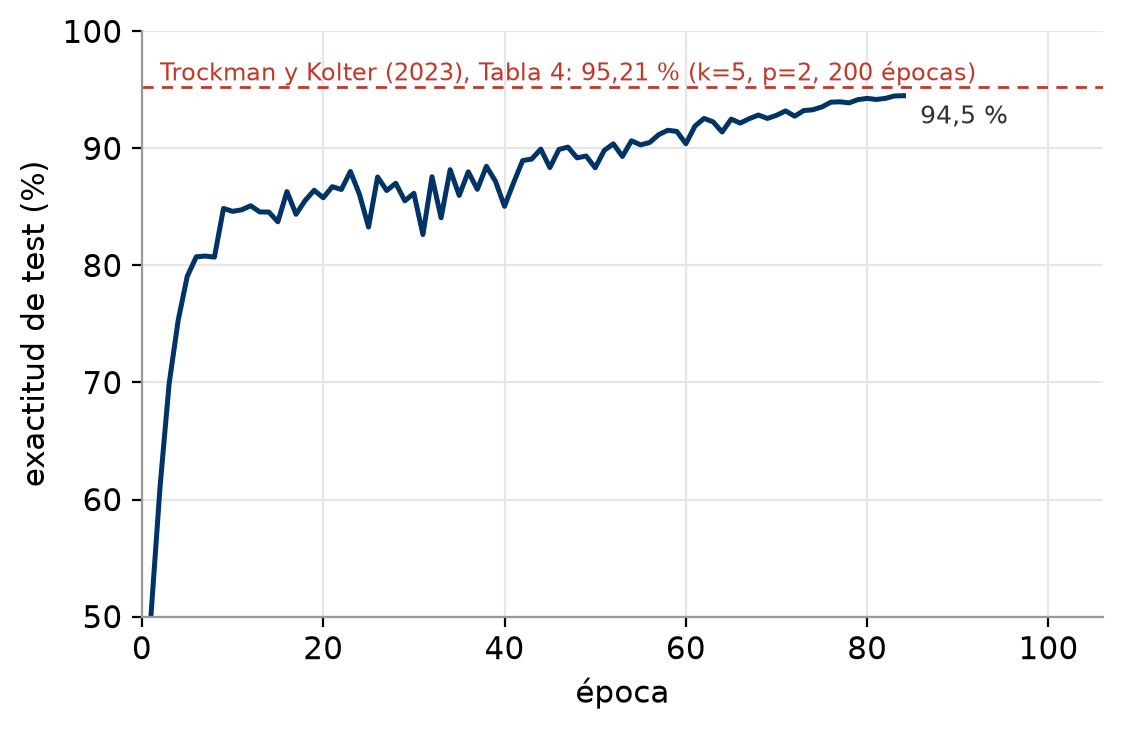
\includegraphics[width=0.62\textwidth]{f_colab.png}
\nota{Exactitud de test por época de ConvMixer-256/8 ($k=5$, $p=2$), sólo para seguimiento: el valor que se informa es el de la última época, sin elegir la mejor. La línea roja es el valor del artículo para la misma configuración con 200 épocas. Elaboración propia con el script \texttt{src/colab\_receta\_paper.py}.}
\end{figure}

\begin{table}[h]\small
\caption{La misma metodología con distinto cómputo: CPU propia, GPU de Colab, GPU de Kaggle y artículo}
\label{tab:cpugpu}
\centering
\resizebox{\textwidth}{!}{\begin{tabular}{lcccc}
\toprule
 & CPU propia (8 núcleos) & Google Colab (T4) & Kaggle (T4) & Artículo (GPU)\\
\midrule
Modelo & 128/8, $k=9$, $p=2$ & 256/8, $k=5$, $p=2$ & 256/8, $k=5$, $p=2$ & 256/8, $k=9$ o $5$, $p=2$\\
Parámetros & 223\,370 & 594\,186 & 594\,186 & 709\,k / 594\,k\\
Aumentación & escalado, recorte y espejo & + RandAugment, ColorJitter, borrado & Colab + mixup y CutMix & \texttt{timm} + mixup y CutMix\\
Weight decay & 0,01 & 0,005 & 0 & 0 (Tabla 4)\\
Épocas & \epocasCNN & \epColab & \epKaggle & 200\\
Tiempo por época & \minEpCPU{} min & \segColab{} s & \segKaggle{} s & no informado\\
Tiempo total & \minCMnueve{} min & \minColab{} min & \minKaggle{} min & no informado\\
Exactitud de test & \pct{\accCMnueve} & \pct{\accColab} & \pct{\accKaggle} & \pct{95,0} / \pct{95,21}\\
\bottomrule
\end{tabular}}
\nota{Una corrida por configuración, sin repetir semillas. Colab y Kaggle: se informa la última época, sin elegir la mejor; ambas con una GPU Tesla T4 (en Kaggle la sesión tenía dos, pero el script usa una). Colab entrenó \colabNota. Valores del artículo: Trockman y Kolter (2023, Tabla 4). Antes de la corrida de Colab que se informa hubo otra idéntica que se cortó en la época 84 (94,50 \%); el registro está en \texttt{results/}.}
\end{table}

La Tabla~\ref{tab:cpugpu} resume la comparación que me parece más interesante para discutir. Hay tres lecturas.
Primero, en un tiempo de reloj parecido (entre 1,5 y 2 horas), la GPU entrenó un modelo 2,7 veces más grande, con
muchas más épocas y con la aumentación completa, y ganó unos 12 puntos con el mismo código. Esto relativiza las
comparaciones entre arquitecturas: una parte de lo que se atribuye a ``un modelo mejor'' corresponde a ``un modelo que
recibió más cómputo y una receta más trabajada''. Es justamente la crítica que se le puede hacer al artículo cuando
compara contra números de otros trabajos.

Segundo, la receta cuenta. Pasar de la receta del repositorio (100 épocas, \pct{\accColab}) a la del artículo (200
épocas, mixup, CutMix y sin \emph{weight decay}) subió la exactitud de \pct{\accColab} a \pct{\accKaggle}, es decir, un
punto, y quedó 0,27 puntos por encima del \pct{95,21} publicado. Con una sola semilla por configuración, esa
diferencia con el artículo está dentro de lo que cabe esperar por azar (del orden de 0,2 a 0,3 puntos), así que lo
prudente es decir que la réplica \emph{iguala} el resultado publicado y no que lo supera. Tampoco puedo separar
cuánto aportó cada cambio (las épocas, mixup y CutMix, o el \emph{weight decay}), porque cambié todo junto; sólo el
artículo muestra que quitar mixup y CutMix casi no cambia el resultado (Tabla 3), lo que sugiere que el grueso viene de
las épocas.

Tercero, el costo. Con la misma GPU, la corrida de Kaggle tardó unos \minKaggle{} minutos (\segKaggle{} s por época)
y la de Colab unos \minColab{} minutos con la mitad de las épocas (\segColab{} s por época): en Kaggle cada época
fue más del doble de rápida. No sé a qué atribuirlo con certeza: la GPU es la misma (Tesla T4), pero cambió la
cantidad de procesos que cargan y aumentan las imágenes (4 en Kaggle y 2 en Colab) y, con RandAugment, esa parte corre
en la CPU y puede ser el cuello de botella. En la práctica, Colab gratuito nos negó la GPU por límite de uso a la
mañana siguiente y había cortado una corrida en la época 84; Kaggle ofrece unas 30 horas semanales y permite dejar la
corrida en segundo plano sin tener la pestaña abierta, lo que la hizo más cómoda y confiable para un entrenamiento
largo.

\textbf{Ablaciones: qué se reprodujo y qué no.}
\begin{itemize}
  \item \emph{Tamaño de parche: se reprodujo.} Con $p=4$ la exactitud cae a \pct{\accCMpcuatro} ($-$\difPatch{}
  puntos frente a $p=2$; en el artículo, $-2{,}4$). Con parches más grandes la resolución interna baja de
  $16\times16$ a $8\times8$ y el modelo pierde detalle, aunque corre unas 3,7 veces más rápido.
  \item \emph{Tamaño de núcleo: no se reprodujo.} Con $k=3$ obtuve \pct{\accCMtres}, es decir,
  \textbf{\difKernelAbs{} puntos a favor del núcleo chico}, al revés que en el artículo ($+2{,}3$ a favor de $k=9$
  con 200 épocas). Mi interpretación es que, con sólo \epocasCNN{} épocas, el modelo con menos parámetros y un sesgo
  local más fuerte converge antes, mientras que los núcleos grandes necesitan más entrenamiento para aprovechar el
  campo receptivo amplio. Los propios autores admiten esta posibilidad (``\emph{It could be that with more training
  iterations or more regularization, the effect of larger kernels would be more pronounced}'', Apéndice~B). Con una
  sola semilla por modelo, una diferencia de 2 puntos es indicativa pero no concluyente.
  \item \emph{ConvMixer frente a ResNet: empate.} La ResNet entrenada con la misma receta obtuvo \pct{\accResNet}
  frente a \pct{\accCMnueve} del ConvMixer ($k=9$), una diferencia de 0,3 puntos, menor que la variabilidad
  esperable entre semillas. El artículo encuentra una ventaja clara del ConvMixer en ImageNet, con modelos 100
  veces más grandes y 150 épocas. En esta escala no la observo.
  \item \emph{Velocidad: se reprodujo.} En inferencia, la ResNet procesa \tputResNet{} imágenes por segundo y el
  ConvMixer con $k=9$ y $p=2$, \tputCMnueve: la ResNet es \ratioTput{} veces más rápida, en línea con las Tablas~1
  y~2 del artículo. El entrenamiento muestra lo mismo: 110 minutos el ConvMixer y 32 minutos la ResNet.
\end{itemize}

\begin{figure}[h]
\caption{Ablaciones de la réplica frente a la Tabla 4 del artículo, y velocidad frente a exactitud}
\label{fig:ablaciones}
\centering
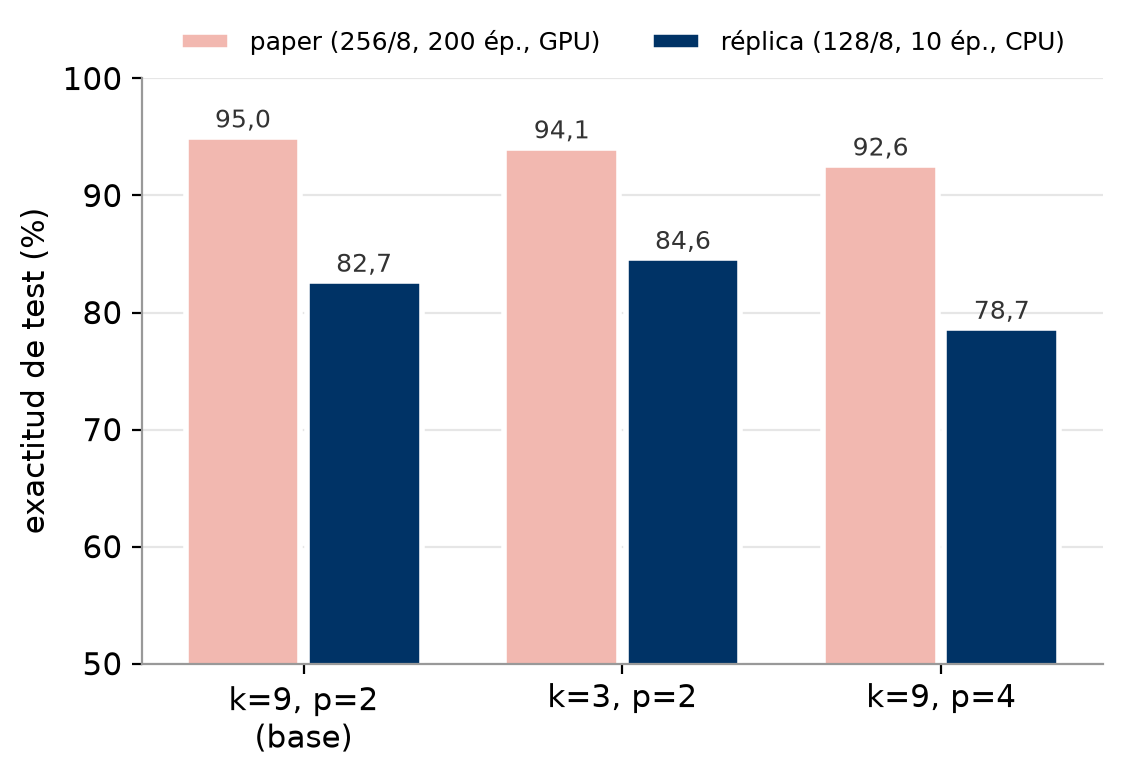
\includegraphics[width=0.49\textwidth]{f_ablaciones.png}\hfill
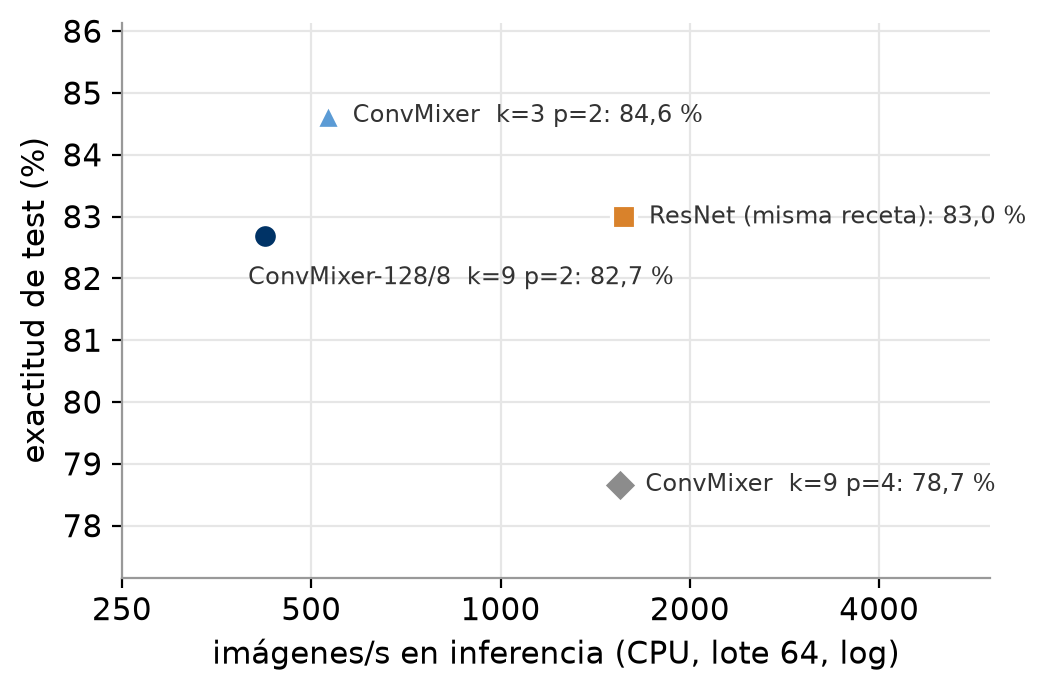
\includegraphics[width=0.49\textwidth]{f_throughput.png}
\nota{Izquierda: exactitud de test de la réplica (ConvMixer-128/8, 10 épocas, CPU) y del artículo (ConvMixer-256/8,
200 épocas, GPU; Trockman y Kolter, 2023, Tabla~4). Derecha: imágenes por segundo en inferencia, medidas en la misma
CPU con lotes de 64 (eje logarítmico). Elaboración propia.}
\end{figure}

\textbf{Los modelos del programa.} El orden de exactitud reproduce el recorrido del curso: perceptrón
(\pct{\accPerceptron}) $\approx$ seudoinversa (\pct{\accLineal}) $<$ ELM (\pct{\accELM}) $<$ MLP
(\pct{\accMLP}) $\ll$ CNN (\pct{\accResNet}--\pct{\accCMtres}). Los dos modelos lineales empatan porque comparten
la misma limitación: una frontera lineal sobre los 3\,072 píxeles. La validación cruzada eligió una regularización
fuerte ($\lambda=\lamCV$), señal de que el sistema está mal condicionado (píxeles vecinos casi colineales). La ELM
mejora al agregar no linealidad, pero sus rasgos aleatorios no aprovechan la estructura espacial; además, con
$N=45\,000\gg L=3\,000$ casi no sobreajusta, y su exactitud seguía subiendo con $L$, de modo que el límite fue la
memoria y no el método. El ML-ELM (\pct{\accMLELM}) quedó por debajo de la ELM simple: sus autoencoders comprimen
los píxeles a 1\,000 dimensiones con una reconstrucción lineal y pierden información útil para clasificar. El MLP,
con 16 veces más parámetros que el ConvMixer, queda 25 puntos abajo y sobreajusta (76\,\% en entrenamiento frente a
58\,\% en validación). Es la mejor ilustración del \emph{sesgo inductivo}: la localidad y los pesos compartidos de
la convolución valen más que los parámetros.

\begin{figure}[h]
\caption{Exactitud de test de todos los modelos de la réplica en CIFAR-10}
\label{fig:barras}
\centering
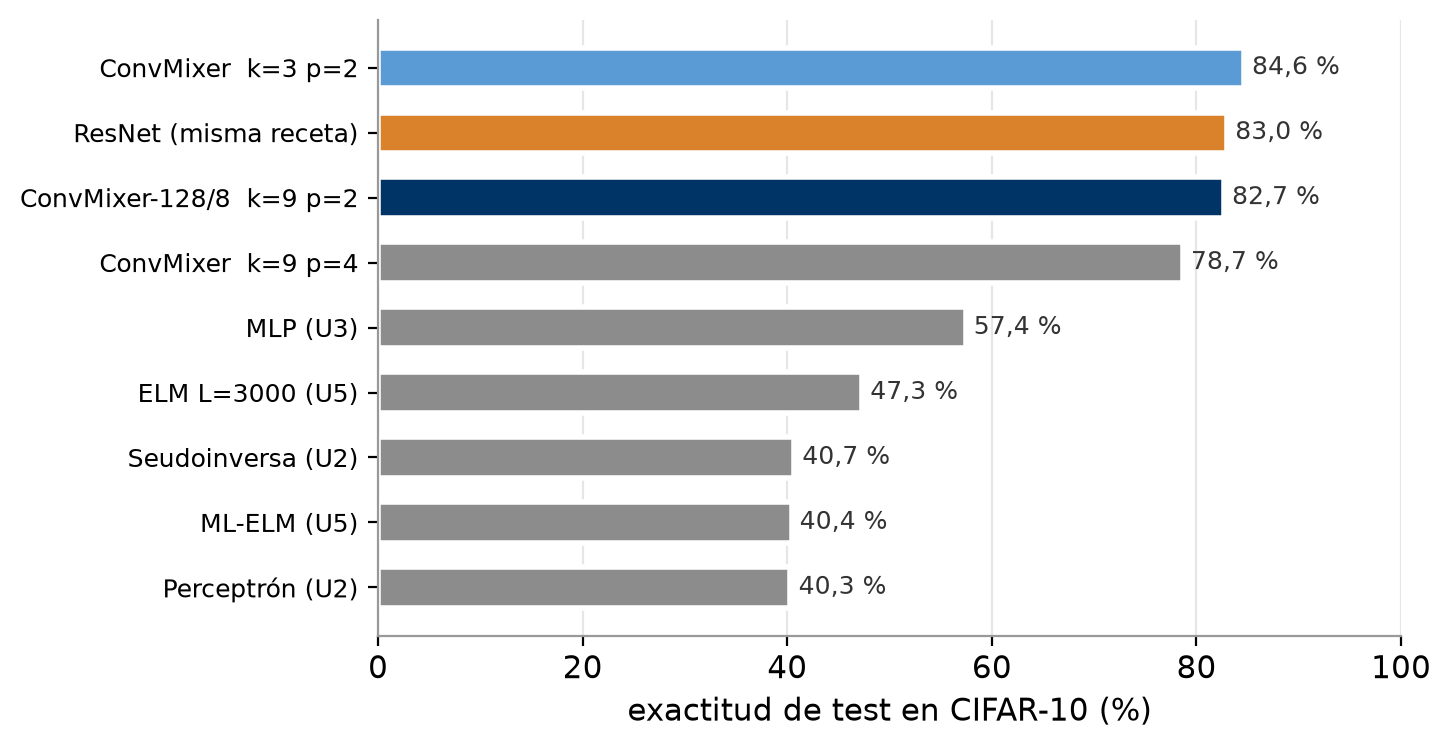
\includegraphics[width=0.75\textwidth]{f_barras.png}
\nota{Azul oscuro: modelo del artículo; naranja: línea de base ResNet; gris: ablaciones y modelos de las unidades 2,
3 y 5. Promedio de 3 semillas en los modelos no convolucionales. Elaboración propia.}
\end{figure}

\textbf{Limitaciones de esta réplica.} Una sola semilla por CNN, por costo de cómputo; 10 épocas; ningún
ajuste de hiperparámetros para la ResNet, igual que en el artículo; y modelos clásicos sobre píxeles crudos, sin
extracción de rasgos. Las diferencias menores a un punto no deben interpretarse.
